% !TEX encoding = UTF-8 Unicode
%%==================================================
%% thanks.tex for SJTU Bachelor Thesis
%% version: 0.5.2
%% Encoding: UTF-8
%%==================================================

\chapter{Empirical Analysis on Stock Market Indices}
\label{chap:positive}

In this chapter we present the numerical results of HMM application for real-world data. 
empirical analysis is conducted on both Chinese and U.S. stock market indices.
We first make several base assumptions on the model and realizations, 
and propose some conjectures on the results, 
including model effectiveness, prediction correctness, 
and possible differences caused by diverse data frequency and observation time period, etc.
We then perform empirical analysis on Standard \& Poor's 500 Index (S\&P 500) and present both 
numerical and visual results in Sec.\,\ref{sec:positive:SP}.
Similar analysis is also carried out on Chinese CSI 300 Index in Sec.\,\ref{sec:positive:CSI}.
We take a further look at the Chinese market and apply the model for data with higher frequencies.
An overall analysis is presented in Sec.\,\ref{sec:positive:result} 
along with comparisons among different data groups.

%%%%%%%%%%%%%%%%%%%%%%%%%%

\section{Assumptions and conjectures}
\label{sec:positive:aspconj}
In this section we specify some basic but necessary assumptions 
for the model application and empirical analysis,
and also propose some conjectures on the prediction result,
including differences in behaviors, potential causes of prediction errors, etc.


\subsection{Assumptions}
\label{sec:positive:aspconj:asp}
The main parameters of a hidden Markov model include 
the state transition matrix and conditional distribution density functions, 
of which dimensions are predetermined by the number of hidden states 
and values are computed through model estimation procedure.

        \begin{asp}
        \label{asp:states}
        The U.S. and Chinese market both have and only have three hidden states,
        namely bear, intermediate and bull.
        \end{asp}
This assumption is intuitively easy to explain.
Usually we tend to describe the market as a bull if the index keeps rising 
and a bear if it goes down all the time.
Sometimes the trend of the index is not that obvious,
daily returns dangle around zero and market volatility is low,
this is when we consider the market as in an intermediate state.
Assuming the market have exactly three states suits customs and has realistic economic meanings.

However, taking the number of states as three might not be statistically optimal,
and we will talk about it in Sec.\,\ref{sec:positive:result:states}.

        \begin{asp}
        \label{asp:distribution}
        Stock returns conditional on the market state are normally distributed.
        Distribution parameters (expectation $\mu$ and variance $\sigma^2$) 
        vary across hidden states and time.
        \end{asp}
Assumption \ref{asp:distribution} follows traditional economic and financial ideas 
and is accepted in most models.
Besides, the normal distribution assumption guarantees the convergence of EM algorithm
and the existence of analytic solution to iterative log-likelihood maximizations 
(see Sec.\,\ref{sec:HMM:EM}).

Some more advanced models have been proposed,
considering the skewness and kurtosis of real-world returns' sample density distribution,
and \cite{Kon:1984ih} presents detailed analysis and comparisons of them.
The topic is beyond the scope of this work so no further discussions will be made,
and we stick to the normal distribution assumption throughout this thesis.


\subsection{Conjectures}
\label{sec:positive:aspconj:conj}
Based on the system described in Sec.\,\ref{sec:system:function},
we propose some conjectures about the model calibration and simulated prediction results.

        \begin{conj}
        \label{conj:lag}
        Prediction results are good at first, and might worsen as processing.
        More specifically, the prediction result may present 
        similar trend and pattern as the historical data that is used for initial model calibration,
        which can be viewed as time lag effect, 
        and that is because the model incorporates too much out-dated information.
        \end{conj}
Conjecture \ref{conj:lag} is one of the potential sources of prediction errors (and maybe the largest).
As described in Sec.\,\ref{sec:system:function:prediction},
every time the prediction processes to the next loop, i.e.\,the next out-of-sample time node,
it takes one more point into the model, but not replaces the oldest one.
Thus, all information in the past still exist, and worse,
all data takes the same weight in the model.
The data from two years ago is as significant as one from yesterday 
when predicting the return of tomorrow, and that is quite against intuition.
Too much weight on out-dated data shall be reflected as time lags in prediction result.
Potential improvement for this problem will be proposed in Sec.\,\ref{sec:future:lag}.

        \begin{conj}
        \label{conj:period}
        Prediction correctness vary with time periods of the data,
        i.e.\,model calibrated for different time periods will have differences in prediction accuracy 
        (ceteris paribus\footnote{Meaning holds all other conditions the same. 
        It is important to do so for results comparisons and to draw meaningful conclusions.}).
        \end{conj}
Conjecture \ref{conj:period} is proposed from the perspective of time.
Although market states switch to each other, 
each state lasts for some time and the endurings are not necessarily short.
Hence, it is very common (almost sure) that the distribution of states 
vary every year (maybe less or more frequently);
even though there should be economy cycles,
hidden market states changed and differed from previous years.
So it is possible that the model have different effectiveness and prediction correctness 
when calibrated with market data from different time period.
We will try to catch the difference by separating data into different time period groups
and applying the model to each group.
Detailed result analysis and comparisons will be given in Sec.\,\ref{sec:positive:result:time}.

Another thing worth mentioning is that the differences between the time groups
could also be supportive evidence for Conjecture \ref{conj:lag}.
Distinguishing the groups also means cutting off data from the previous time period,
and the results from the sub-periods and those from the entire sample period may differ.
However, the ``support'' here can hardly meet the requirement of ceteris paribus.
We merely provide a point of view here and further analysis and experiments 
should be conducted if to prove this opinion,
which is not the major concern of this thesis.


        \begin{conj}
        \label{conj:frequency:states}
        Global decoding results may vary with data frequency.
        For a certain time period, 
        hidden states sequence may be found different using data with diverse frequency.
        \end{conj}

        \begin{conj}
        \label{conj:frequency:prediction}
        Prediction results may vary with data frequency.
        More specifically, data with higher frequency may generate better prediction results.
        \end{conj}
Conjecture \ref{conj:frequency:states} and \ref{conj:frequency:prediction} 
are concerned with data frequency within the same time period.
For data within the same time period,
difference in observation frequencies represents different amount of information.
Usually is the case that the higher the frequency is, the more information the data contains.
Thus we can also examine the differences due to various observation frequencies.
To be more specific, we suppose that prediction correctness increase with data frequency.
Examination of these two conjectures will be given in Sec.\,\ref{sec:positive:result:frequency}.

%%%%%%%%%%%%%%%%%%%%%%%%%%

\section{U.S. S\&P 500 Index daily return series}
\label{sec:positive:SP}
S\&P 500 is one of the oldest and the most important stock market indices in the world, 
and it is safe to say that it has the most typical behaviors of a mature stock market. 
We firstly apply our model to S\&P 500 and then CSI 300 so as to 
compare the effectiveness of our model under different market maturity.


\subsection{Data preprocessing and description}
\label{sec:positive:SP:data}

        \begin{figure}[!hbt]
        \center
        \includegraphics[width=\textwidth]{SP500/histFig1.pdf}
        \caption{S\&P 500 historical prices}
        \label{fig:SP:hist}
        \end{figure}
Sample data of S\&P 500 is composed of its daily close 
between Mar. $5^{th}$, 2013 and Mar. $4^{th}$, 2016
\footnote{Data source: Yahoo Finance},
i.e.\,757 prices within three years in total. 
Of all 757 records, two thirds of them (data before Mar. $6^{th}$, 2015) are used as in-sample data
for K-Means model training and HMM initialization. 
The remaining one third are reserved to compare with the simulated prediction results.

Illus.\,\ref{fig:SP:hist} presents the historical prices and trends of S\&P 500 during all three years. 
The index had been going up steadily, though with fluctuations, 
since the very beginning until around July, 2015. 
It then suffered a large downturn followed by a short period of turbulence, 
and then a large upgoing trend.
Generally speaking, the index presented quite different behaviors, 
in terms of both trend and volatility, between in-sample data and out-of-sample data.

        \begin{figure}[!hbt]
        \center
        \includegraphics[width=\textwidth]{SP500/histFig3.pdf}
        \caption{S\&P in-sample trend with daily return bars}
        \label{fig:SP:histin}
        \end{figure}

        \begin{figure}[!hbt]
        \center
        \includegraphics[width=\textwidth]{SP500/histFig4.pdf}
        \caption{Density distribution of S\&P in-sample daily returns}
        \label{fig:SP:ret}
        \end{figure}
Now take a look at the in-sample period.
Density distribution of daily returns is almost bell-curve shaped,
with slight skewness to the right (see Illus.\,\ref{fig:SP:histin} and \ref{fig:SP:ret}). 
Almost all returns are within the range $[-2.5\%,2.5\%]$ and 
with 5-day volatility less than $2\%$ (daily basis, indicated in Illus.\,\ref{fig:SP:KMeans}).

        \begin{figure}[!hbt]
        \center
        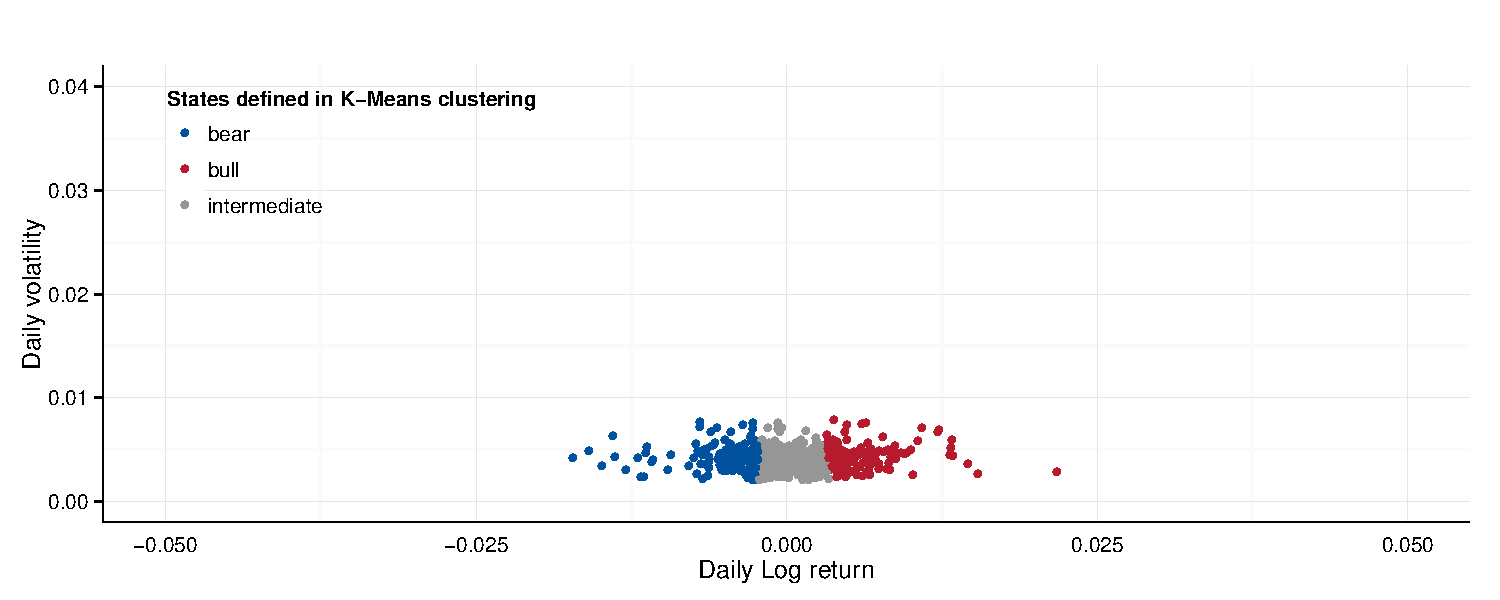
\includegraphics[width=\textwidth]{SP500/histFig2.pdf}
        \caption{K-Means result of S\&P 500 in-sample returns}
        \label{fig:SP:KMeans}
        \end{figure}
The result of K-Means clustering is pretty straightforward 
as it classifies the lowest one third of the returns as bear,
the highest one third as bull and the remaining as in the intermediate state.
Note that the clustering of K-Means method is purely based on quantitative differences of the data
(daily return and corresponding 5-day volatility in this case),
and has nothing to do with the market states then.
The definition and names of the states are artificially given to 
merely distinguish the three clustering centers.


\subsection{State transition parameters}
\label{sec:positive:SP:transition}
The three by three state transition matrix has nine unknown parameters in total,
estimated by EM algorithm through iteration.
Illus.\,\ref{fig:SP:transition} presents four chord plots
of the state transition matrix for S\&P 500 in-sample data.

        \begin{figure}[!hbt]
        \center
        \includegraphics[width=\textwidth]{SP500/transFig1.pdf}
        \caption{State transition for S\&P 500 in-sample data}
        \label{fig:SP:transition}
        \end{figure}
The first plot in Illus.\,\ref{fig:SP:transition} visualizes a complete state transition matrix.
Three different colors each stands for a hidden state.
Every chord links two arcs:
the arc with the same color as the chord represents the current state,
and the other one represents the next state.
Since HMM allows for stays of the latent variable,
the state transition matrix may have non-zero diagonal entries,
leading to chords that travels from and to the same arc.

The latter three plots each shows the transition vector conditional on the current state.
As can be seen, a bull market is most likely to enter a bear state (with probability of $42\%$),
and to stay put or transit into an intermediate state with the same probability (of $29$\%).
However, a market at intermediate state stays at intermediate with great chance (about $93\%$),
but is almost impossible to change into a bull market (with probability less than $10^{-5}$).
A bear market, on the other hand, is more likely to transit into a bull than stay still 
with a slightly higher probability ($55\%$ vs. $45\%$) 
and has very little chance to go intermediate (with probability less than $10^{-6}$).
Transitions between extreme cases (bull and bear) seem more likely to happen,
compared to transitions between the intermediate state and an extreme case.

These patterns indicate a highly volatile market, 
where it is more possible to meet with a rebounce rather than a trend 
(except the intermediate state, which might represent lack of trends).
This fact can be indirectly proved by Illus.\,\ref{fig:SP:histin}.
The index kept going up for two years and the trend seems quite obvious;
but upturns and downturns, not only small waves but also large ones, 
are densely distributed within the period.
The volatility of the market will be more clear if one takes into account inflation.


\subsection{Conditional distribution parameters}
\label{sec:positive:SP:distribution}
Another type of unknown parameters are those of the Gaussian distributions 
conditional on each hidden state.
Conditional distribution parameters include three pairs of 
expectation and variance (or standard deviation).
The optimal estimation during each iteration can be analytically computed through EM
(see Sec.\,\ref{sec:HMM:EM}).

The estimation result of S\&P 500 in-sample is given as follow:
        \begin{equation}
        \left (
        \begin{array}{c c c}
        -1.13\%  &  -0.08\%  &  0.78\%  \\
         0.70\%  &   0.49\%  &  0.65\%  \\
        \end{array}
        \right ).
        \end{equation}
Each column in order represents the bear state, the intermediate and the bull.
Entries in the first row are corresponding expectations 
and ones in the second row are standard deviations.
It is clear that returns during the bear and bull 
have higher variances and non-zero expectations,
while returns during the intermediate are closer to zero and have lower volatility.

        \begin{figure}[!hbt]
        \center
        \includegraphics[width=\textwidth]{SP500/paramFig1.pdf}
        \caption{Conditional distribution parameters across time}
        \label{fig:SP:distscatter}
        \end{figure}
We also consider time-variation of the parameters.
As a matter of fact, when the simulated prediction is processing,
more information has been incorporated into the model and parameters change with time.
Illus.\,\ref{fig:SP:distscatter} and \ref{fig:SP:distdist} are to 
describe the conditional distribution parameters time series.

The aforementioned patterns about the parameters remain across time.
Bear(bull) states have expected returns significantly below(over) zero and higher volatility,
while intermediate states have expectations around zero and a relatively lower volatility.
Notice that some distributions conditional on bull states also have smaller variance,
indicating a slower and milder rise.
Clearly bears always come more strongly.

        \begin{figure}[!hbt]
        \center
        \includegraphics[width=\textwidth]{SP500/paramFig2.pdf}
        \caption{Density distribution of conditional distribution parameters}
        \label{fig:SP:distdist}
        \end{figure}
Illus.\,\ref{fig:SP:distdist} shows the density distribution of these parameters.
The multi-modality of $\sigma$ matches the multi-clustering-center in Illus.\,\ref{fig:SP:distscatter}.
Therefore, chances are that even the same hidden state presents different behaviors.
It means it might be necessary to increase the number of hidden states in the model,
which is currently against Assumption \ref{asp:states} and 
will be discussed about in Sec.\,\ref{sec:positive:result:states}.


\subsection{Global decoding and hidden states}
\label{sec:positive:SP:states}

        \begin{figure}[!hbt]
        \center
        \includegraphics[width=\textwidth]{SP500/statesFig1.pdf}
        \caption{S\&P 500 in-sample trend and states sequence}
        \label{fig:SP:seqstates}
        \end{figure}
Global decoding based on Viterbi algorithm enables us to find the 
most probable sequence of hidden states,
which shall help us learn about the market with ability to 
identify the market states during the observation period.

Illus.\,\ref{fig:SP:seqstates} provides knowledge about 
the sequence of hidden states of S\&P 500 in-sample data.
The color gray, standing for the intermediate state, 
makes up the majority of the figure.
Bears and bulls are far less frequent than intermediates and often come together.
This phenomenon is better expressed by Illus.\,\ref{fig:SP:states}

        \begin{figure}[!hbt]
        \center
        \includegraphics[width=\textwidth]{SP500/statesFig2.pdf}
        \caption{S\&P 500 historical hidden states}
        \label{fig:SP:states}
        \end{figure}
The upper two parts of Illus.\,\ref{fig:SP:states} are almost the same except for color labels,
which proves the closeness of bears and bulls.

Actually the global decoding result also supports, from a visual perspective, 
our findings mentioned in Sec.\,\ref{sec:positive:SP:transition},  
that extreme states tend to transit into each other instead of the intermediate.

        \begin{figure}[!hbt]
        \center
        \includegraphics[width=\textwidth]{SP500/statesFig3.pdf}
        \caption{Comparison between K-Means states and HMM hidden states}
        \label{fig:SP:diffstates}
        \end{figure}
Illus.\,\ref{fig:SP:diffstates} shows the states of in-sample returns implied by HMM and K-Means.
As we mentioned before, K-Means distinguish the states based merely on 
quantitative properties of the data, not taking into account their correlations and transitions.
Hence, most of the differences lie in the bull zone in K-Means, 
which are identified as intermediate in HMM.
Statistically speaking, these returns are relatively higher,
but they are more likely to appear during an intermediate state according to HMM.
It is similar for those which are labeled as bear in K-Meas but intermediate in HMM.
There also exist some points classified as intermediate in K-Means 
but considered to be in one of the extreme states in HMM.
These points may be viewed as small adjustments (or small rebounces) under a big trend,
even though they are close to zero.


\subsection{Simulated prediction results}
\label{sec:positive:SP:prediction}
Simulated prediction is carried out on out-of-sample data and 
the model is updated on a daily basis.
Information of the real historical daily return is incorporated into 
the current model in order to predict the return for the next day.
Illus.\,\ref{fig:SP:predictionall} presents the result of the prediction
over the entire observation period (in-sample and out-of-sample).
Predicted returns are cumulatively summed and taken exponential, 
multiplied by the first closing price of the out-of-sample data.

        \begin{figure}[!hbt]
        \center
        \includegraphics[width=\textwidth]{SP500/predictionFig1.pdf}
        \caption{S\&P 500 simulated prediction result}
        \label{fig:SP:predictionall}
        \end{figure}
Visually speaking the prediction result is extremely poor.
The predicted result preserves the trend of the in-sample data
and has started to deviate from the real history since June 2015.

        \begin{figure}[!hbt]
        \center
        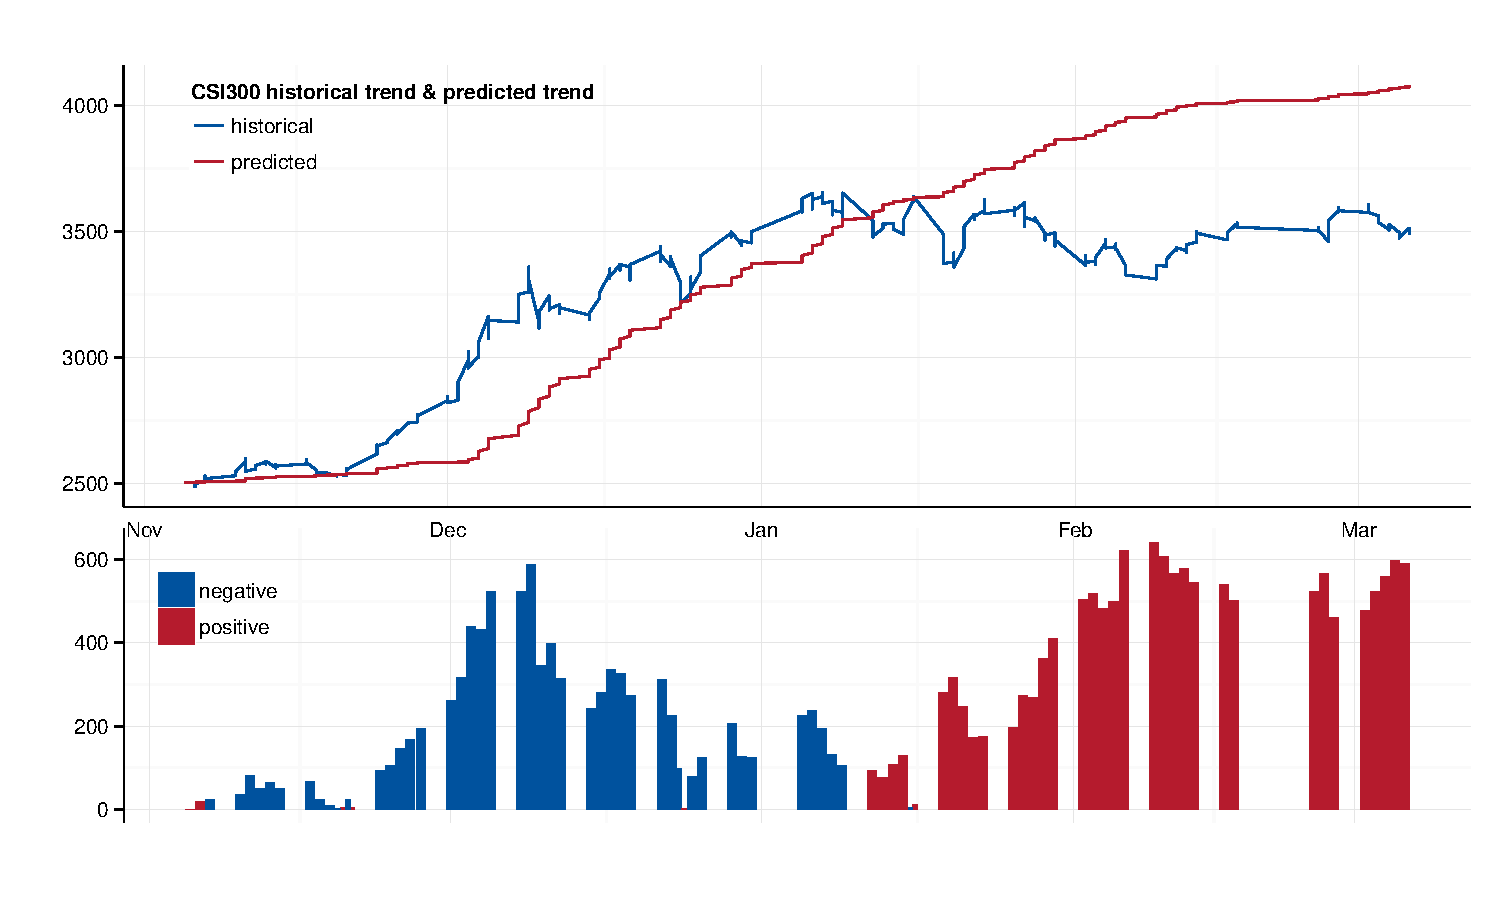
\includegraphics[width=\textwidth]{SP500/predictionFig2.pdf}
        \caption{S\&P 500 simulated prediction result out-of-sample part}
        \label{fig:SP:predictionout}
        \end{figure}
Illus.\,\ref{fig:SP:predictionout} shows both the trend and differences 
between the historical value and the prediction result.
Difference shot up when the index changed from a up-going trend to a downward shape.
Illus.\,\ref{fig:SP:predictionstd} indicates that even considering the standard deviations 
cannot help with the prediction.

        \begin{figure}[!hbt]
        \center
        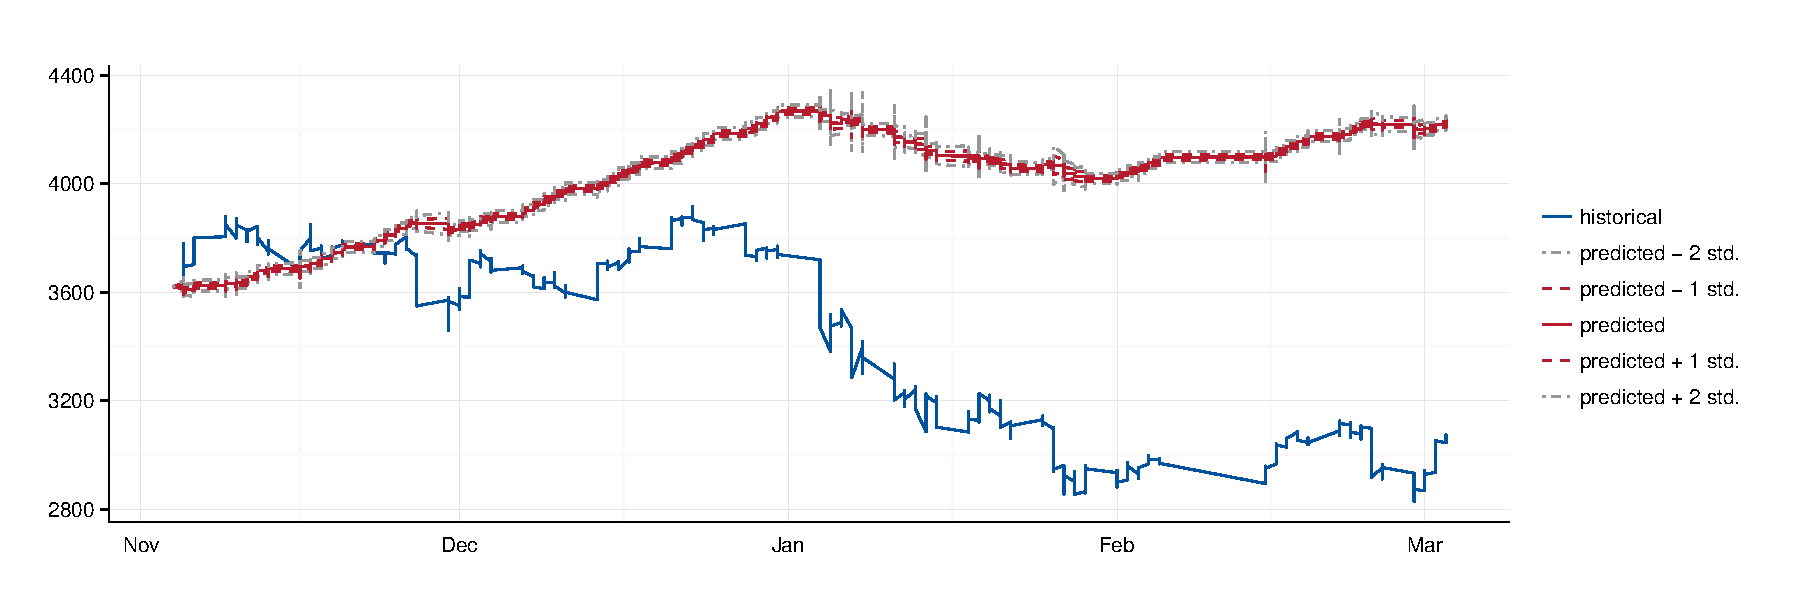
\includegraphics[width=\textwidth]{SP500/predictionFig3.pdf}
        \caption{S\&P 500 simulated prediction result with confidence band}
        \label{fig:SP:predictionstd}
        \end{figure}
However, the simulated prediction result has a win ratio of $50.4\%$,
which means the model has predicted the right direction of the index 
with probability slightly over a half.

Besides, as we mentioned in the very beginning of Sec.\,\ref{sec:positive:SP:prediction},
the predicted curve is based on the first closing price of the out-of-sample data 
but does not consider the current price of the index.
The most direct and obvious result of such a method is that prediction errors accumulate,
leading to larger and larger deviation from the real history.

        \begin{figure}[!hbt]
        \center
        \includegraphics[width=\textwidth]{SP500/predictionFig4.pdf}
        \caption{S\&P 500 adaptive prediction}
        \label{fig:SP:predictiondyn}
        \end{figure}
Therefore, it is reasonable to fully use the information provided by the data,
including both real returns and real closing prices.
We base prediction for the next day on both return and closing price at the standing point,
and the result seems much better, as shown in Illus.\,\ref{fig:SP:predictiondyn}.
Illus.\,\ref{fig:SP:predictiondynstd} plots the result and index along with 
$\pm \sigma, \pm 2\sigma$ bands.
The real index is almost entirely covered by the $\pm 2\sigma$ band,
which stands for a $95.45\%$ confidence interval of prediction.

        \begin{figure}[!hbt]
        \center
        \includegraphics[width=\textwidth]{SP500/predictionFig5.pdf}
        \caption{S\&P 500 adaptive prediction with confidence band}
        \label{fig:SP:predictiondynstd}
        \end{figure}
It is worth noticing that there are clearly lags 
in the prediction results compared to the real index.
The extension of previous trend in Illus.\,\ref{fig:SP:predictionall} can be viewed
as a stronger version of such lag.
Furthermore, the lagging effect is not relived as time goes by,
but, on the opposite, exacerbated.

Thus, Conjecture \ref{conj:lag} seems reasonable to explain the phenomenon,
that too much outdated information is included and causes the lag and error.
Previous trends extend and too few weights have been allocated for the status quo.
More detailed analysis and explanations will be discussed in 
both Sec.\,\ref{sec:positive:result:prediction} and Sec.\,\ref{sec:future:lag}.

%%%%%%%%%%%%%%%%%%%%%%%%%%

\section{Chinese CSI 300 Index daily return series}
\label{sec:positive:CSI}
Of all stock market indices like Shanghai Composite Index, CSI 500 and CSI 800, etc.,
CSI 300 is the most typical and used for analysis.

\subsection{Data preprocessing and description}
\label{sec:positive:CSI:data}

        \begin{figure}[!hbt]
        \center
        \includegraphics[width=\textwidth]{daily/histFig1.pdf}
        \caption{CSI 300 historical prices}
        \label{fig:CSI:hist}
        \end{figure}
Sample data of CSI 300 is selected between Mar.\,$5^{th}$, 2013 and Mar.\,$3^{rd}$, 2016
\footnote{Data source: Wind. All data of CSI 300, 
with different frequencies, are from the same data source},
totally 729 prices within three years, 
of which two thirds are used as in-sample, similar to the scheme in Sec.\,\ref{sec:positive:SP}. 
The time period is chosen as the same to the S\&P 500 case as well
so that the results are comparable.

As is shown in Illus.\,\ref{fig:CSI:hist},
the index was almost flat during 2013 and 2014 and met its big upturn at the end of 2014.
The big rise came in two parts and reached peak in May 2015,
followed by a rapid and large fall.
Rebounce occurred around September 2015 and then came another downturn in December.

        \begin{figure}[!hbt]
        \center
        \includegraphics[width=\textwidth]{daily/histFig3.pdf}
        \caption{CSI 300 in-sample trend with daily return bars}
        \label{fig:CSI:histin}
        \end{figure}

        \begin{figure}[!hbt]
        \center
        \includegraphics[width=\textwidth]{daily/histFig4.pdf}
        \caption{Density distribution of CSI 300 in-sample daily returns}
        \label{fig:CSI:ret}
        \end{figure}
The long period of fluctuation and almost half of the upgoing period
makes up the in-sample period.
Density distribution of daily returns has a lower skewness than S\&P 500 in-sample data,
but a longer tail on the left.

\subsection{State transition parameters}
\label{sec:positive:CSI:transition}
State transition matrix of CSI 300 data is quite similar to 
the one in Sec.\,\ref{sec:positive:SP:transition} but different in exact numbers.

        \begin{figure}[!hbt]
        \center
        \includegraphics[width=\textwidth]{daily/transFig1.pdf}
        \caption{State transition for CSI 300 in-sample data}
        \label{fig:CSI:transition}
        \end{figure}
Illus.\,\ref{fig:CSI:transition} implements a similar chord diagram to 
visually present the transition matrix.
A bull market tends to stay at bull or transit into an indermediate with the same probability ($46\%$)
and is relatively unlikely to go into a bear directly.
An intermediate market has the chance of $86\%$ to stay put and 
a slightly higher probability to go into bear ($7.7\%$).
However, a bear market is very likely to get off the status quo,
with a probability of $47\%$ to turn into an intermediate and 
$46$ to even go into a bull directly.
This pattern is quite different from one in the U.S. market.

        \begin{figure}[!hbt]
        \center
        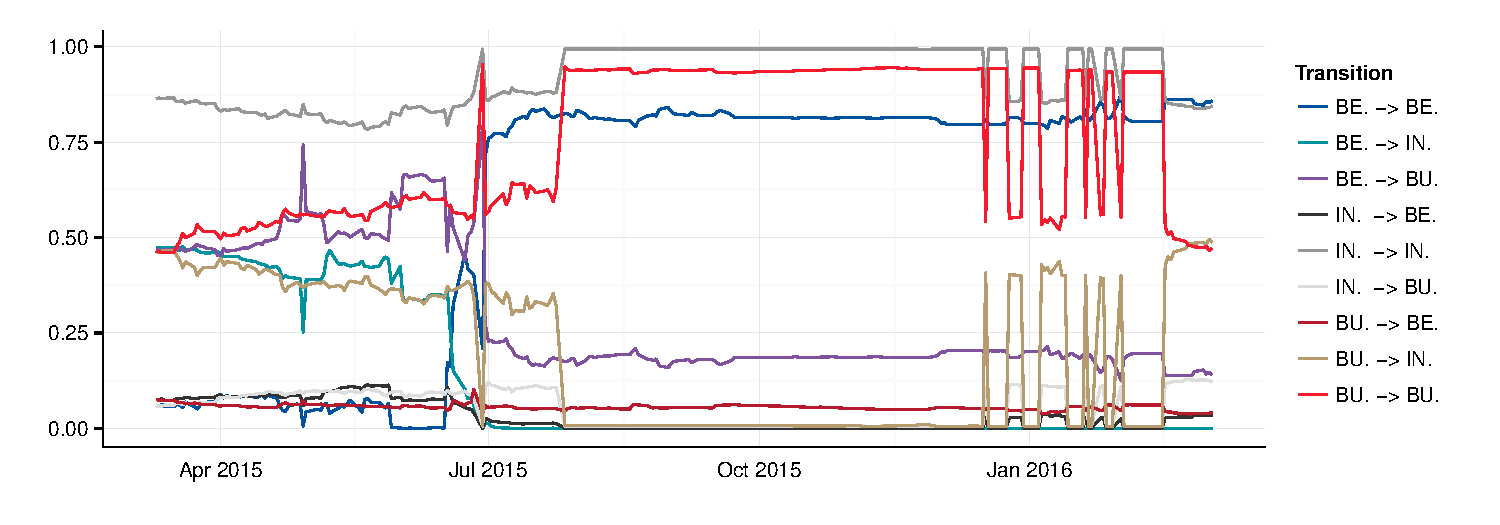
\includegraphics[width=\textwidth]{daily/transFig2.pdf}
        \caption{Evolution of state transition matrix entries}
        \label{fig:CSI:transitionevo}
        \end{figure}

        \begin{figure}[!hbt]
        \center
        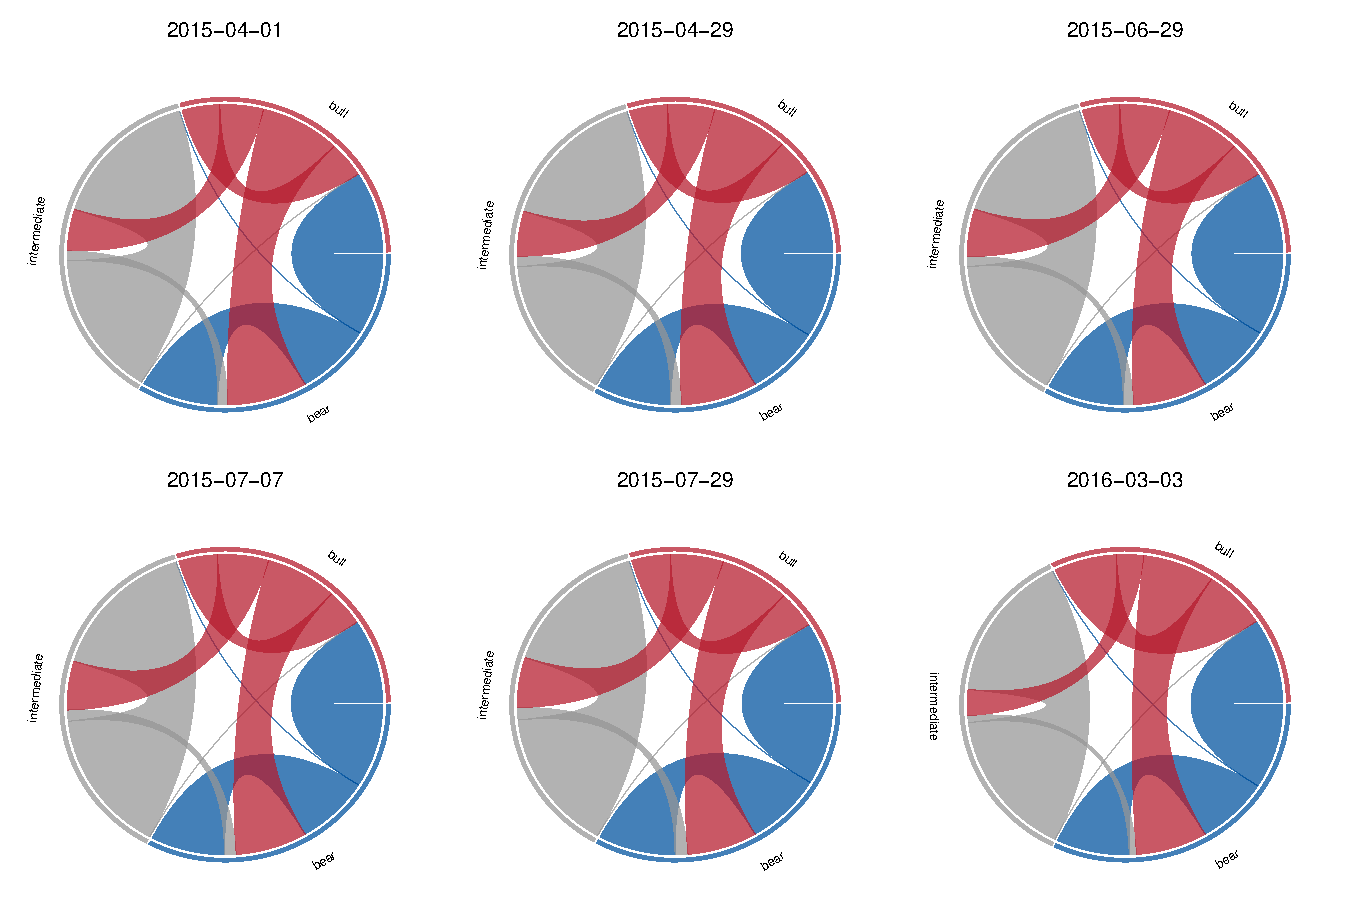
\includegraphics[width=\textwidth]{daily/transFig3.pdf}
        \caption{Typical state transition matrices during the entire period }
        \label{fig:CSI:transitiontypical}
        \end{figure}
To be more thorough, we also examine evolution of the state transition matrix
as the prediction processes, which leads to increases in data used to estimate parameters.
Illus.\,\ref{fig:CSI:transitionevo} plots the dynamic evolution of 
the matrix as size of in-sample data grows.
Dense fluctuations appear in June to July 2015, when the market has just passed its peak,
and in early this year, when another downturn took place.
It seems that falls of the market have greater impacts on the parameters than rises,
and that may be related to the long tail we mentioned in Sec.\,\ref{sec:positive:CSI:data}.

Illus.\,\ref{fig:CSI:transitiontypical} selects six chord diagrams within the entire observation period.
Market states tend to remain the same with more chance after the big fall and
hence the probability to transit into other states goes down,
that is, the market has a bigger tendency to behave like previous trading days.


\subsection{Conditional distribution parameters}
\label{sec:positive:CSI:distribution}
The estimation result of conditional distribution parameters for
CSI 300 in-sample is given as follow:
        \begin{equation}
        \left (
        \begin{array}{c c c}
        -1.66\%  &  0.13\%  &  2.13\%  \\
         1.02\%  &  0.99\%  &  1.23\%  \\
        \end{array}
        \right ).
        \end{equation}
Columns stand for states, the first row for expectation and the second for standard deviation.
The pattern resembles the one in \ref{sec:positive:SP:distribution} and clearly makes sense.


        \begin{figure}[!hbt]
        \center
        \includegraphics[width=\textwidth]{daily/paramFig1.pdf}
        \caption{Conditional distribution parameters across time}
        \label{fig:CSI:distscatter}
        \end{figure}

        \begin{figure}[!hbt]
        \center
        \includegraphics[width=\textwidth]{daily/paramFig2.pdf}
        \caption{Density distribution of conditional distribution parameters}
        \label{fig:CSI:distdist}
        \end{figure}
Illus.\,\ref{fig:CSI:distscatter} and \ref{fig:CSI:distdist} give 
the time-variation of distribution parameters.
High volatility of bears seems more significant than S\&P 500 case, 
but standard deviations are dispersed, 
which is reflected as flatness of the blue line in the downer part of Illus.\,\ref{fig:CSI:distdist}.
Multi-modality exists, indicating changes of the states and 
a potential need to increase the number of hidden states in the model.


\subsection{Global decoding and hidden states}
\label{sec:positive:CSI:states}

        \begin{figure}[!hbt]
        \center
        \includegraphics[width=\textwidth]{daily/statesFig1.pdf}
        \caption{CSI 300 in-sample trend and states sequence}
        \label{fig:CSI:seqstates}
        \end{figure}
Global decoding result meets our expectation well.
The intermediate state lasts for almost two years,
followed by frequent occurences of bulls.
Then there came the large bear until the rebounce,
and then the bear hit the market again.

        \begin{figure}[!hbt]
        \center
        \includegraphics[width=\textwidth]{daily/statesFig2.pdf}
        \caption{CSI 300 historical hidden states}
        \label{fig:CSI:states}
        \end{figure}
The bull states have not appeared consecutively like the bear.
We suppose that is because when the market went up,
the returns were relatively small, 
and small positive returns accumulated to form a long-term bull with help of time,
while the bear came with large negative returns and conquered the market rapidly.
Results visualizations are presented in 
Illus.\,\ref{fig:CSI:seqstates} and \ref{fig:CSI:states}.

        \begin{figure}[!hbt]
        \center
        \includegraphics[width=\textwidth]{daily/statesFig3.pdf}
        \caption{Comparison between K-Means states and HMM hidden states}
        \label{fig:CSI:diffstates}
        \end{figure}
Similarly, differences between HMM states and K-Means states are examined 
(see Illus.\,\ref{fig:CSI:diffstates}).
Differences occur mainly in the bear zone, some in the bull, and few in the intermediate.
The pattern resembles one in Sec.\,\ref{sec:positive:SP:states} and 
we no longer repeat it here.


\subsection{Simulated prediction results}
\label{sec:positive:CSI:prediction}

        \begin{figure}[!hbt]
        \center
        \includegraphics[width=\textwidth]{daily/predictionFig1.pdf}
        \caption{CSI 300 simulated prediction result}
        \label{fig:CSI:predictionall}
        \end{figure}
Simulated prediction result along with CSI 300 in-sample data
is plotted in Illus.\,\ref{fig:CSI:predictionall}.
The out-of-sample part is separatedly presented with daily return bars
in Illus.\,\ref{fig:CSI:predictionout}

        \begin{figure}[!hbt]
        \center
        \includegraphics[width=\textwidth]{daily/predictionFig4.pdf}
        \caption{CSI 300 simulated prediction result out-of-sample part}
        \label{fig:CSI:predictionout}
        \end{figure}
The win ratio of the prediction is $50.2\%$, almost the same as in S\&P case,
and the extension and lagging pattern is more clearly conveyed.
At the very first of the out-of-sample period, 
the predicted index remains going up straight but with a lower slope,
which extends the trend before and also influenced by recent adjustments.
Downturn appears after the real fall takes place and the lag is quite obvious.
Prediction behaviors are similar in the rest part.
Confidence bands and adaptive prediction results are also visualized and 
the formats are similar as in S\&P case.
In order to avoid unnecessary information, 
we do not present the illustrations here and they will be listed in 
Appendix \ref{app:fig} in case the reader is interested
\footnote{Similar prediction and analysis are also carried out for 
CSI 300 data with medium frequencies 
(see Sec.\,\ref{sec:positive:CSI60} and Sec.\,\ref{sec:positive:CSI10},
and the figures are also presented in Appendix \ref{app:fig})}.

However, results are quite good for adaptive predictions.
Though the time lag effect still exists, 
it eliminates the error accumulation on the absolute level of the index.

%%%%%%%%%%%%%%%%%%%%%%%%%%

\section{Chinese CSI 300 Index medium frequency (60min) return series}
\label{sec:positive:CSI60}
CSI 300 medium frequency (60min) return data are selected within 
the same observation period as before.
The only difference is the observation frequency.
Higher frequency indicates that the number of data increase during the same period,
so we split the entire period into three parts,
each has length of about one year (from March to March).


\subsection{Global decoding and hidden states}
\label{sec:positive:CSI60:states}
        \begin{figure}[!hbt]
        \begin{center}
        \subfigure[Mar. 2013 $\sim$ Mar. 2014]
            {\includegraphics[width=0.49\textwidth]{60min_1314/statesFig1.pdf}}
        \subfigure[Mar. 2014 $\sim$ Mar. 2015]
            {\includegraphics[width=0.49\textwidth]{60min_1415/statesFig1.pdf}}
        \end{center}
        \subfigure[Mar. 2015 $\sim$ Mar. 2016]
            {\includegraphics[width=0.49\textwidth]{60min_1516/statesFig1.pdf}}
        \caption{CSI 300 60min data global decoding results}
        \label{fig:CSI60:states}
        \end{figure}
Decoding results in year 2013 to 2014 matches our expectation,
while the result in the latter two sub-periods is quite astonishing.

The last part in Part (b) of Illus.\,\ref{fig:CSI60:states} presents 
the trend of a lasting rise but is identified as bear.
The conditional distribution parameters (60min basis
\footnote{The returns are calculated on a 60min basis and 
we do not annualize the data or change the scale to the same as former cases,
since compared to the actual value of the parameters,
we care more about their differences, orders and decoding and prediction results.}
) in the period are
        \begin{equation}
        \left (
        \begin{array}{c c c}
        0.108\%  &  0.019\%  &  0.115\%  \\
        1.207\%  &  0.324\%  &  0.827\%  \\
        \end{array}
        \right ).
        \end{equation}
The parameter pair corresponding to bear states has a positive expectation
and a relatively big standard deviation.
Thus, the ``bear'' state here has actually a higher expected return than the
intermediate state and is classified as bear because its volatility is higher
and expected return is lower than the bull.

As we mentioned before, 
the name of states here are artificially given to the states based on customs.
During Mar. 2014 to Mar. 2015, 
the market is at a (conventionally acknowledges) bull state almost all the time
and does not actually have a bear state, if not consider the small rebounces.
Therefore, although the labels do not meet our expectations,
the actual distributions are not that unexpected.


\subsection{Simulated prediction results}
\label{sec:positive:CSI60:prediction}
        \begin{figure}[!hbt]
        \begin{center}
        \subfigure[Mar. 2013 $\sim$ Mar. 2014]
            {\includegraphics[width=0.49\textwidth]{60min_1314/predictionFig5.pdf}}
        \subfigure[Mar. 2014 $\sim$ Mar. 2015]
            {\includegraphics[width=0.49\textwidth]{60min_1415/predictionFig5.pdf}}
        \end{center}
        \subfigure[Mar. 2015 $\sim$ Mar. 2016]
            {\includegraphics[width=0.49\textwidth]{60min_1516/predictionFig5.pdf}}
        \caption{CSI 300 60min data simulated prediction results}
        \label{fig:CSI60:prediction}
        \end{figure}
Win ratios in the three year are $51.7\%$, $55.5\%$ and $50.5\%$ separately,
which are all better than former cases.
Time lag effects and error accumulations exist for long-term prediction.
Adaptive prediction results are much better.

%%%%%%%%%%%%%%%%%%%%%%%%%%

\section{Chinese CSI 300 Index medium frequency (10min) return series}
\label{sec:positive:CSI10}
CSI 300 medium frequency (10min) return data have exactly the same structure as 60min data
except higher observation frequency.
This only difference enables us to examine the effect of observation frequency,
or data density within a given time period,
on the decoding results and prediction results.

\subsection{Global decoding and hidden states}
\label{sec:positive:CSI10:states}
        \begin{figure}[!hbt]
        \begin{center}
        \subfigure[Mar. 2013 $\sim$ Mar. 2014]
            {\includegraphics[width=0.49\textwidth]{10min_1314/statesFig1.pdf}}
        \subfigure[Mar. 2014 $\sim$ Mar. 2015]
            {\includegraphics[width=0.49\textwidth]{10min_1415/statesFig1.pdf}}
        \end{center}
        \subfigure[Mar. 2015 $\sim$ Mar. 2016]
            {\includegraphics[width=0.49\textwidth]{10min_1516/statesFig1.pdf}}
        \caption{CSI 300 10min data global decoding results}
        \label{fig:CSI10:states}
        \end{figure}
Anomaly in 10min case occurs in year 2015 to 2016 (instead of 2014 to 2015 in 60min case).
Conditional distribution parameters (10min basis) are
        \begin{equation}
        \left (
        \begin{array}{c c c}
        -0.117\%  &  0.026\%  &  -0.031\%  \\
         1.627\%  &  0.269\%  &   0.515\%  \\
        \end{array}
        \right ).
        \end{equation}
So it is actually very similar to the 60min case,
just that the ``bull'' has a negative expected return and higher volatility here
while the anomaly in 60min case is related to the ``bear'' then.

\subsection{Simulated prediction results}
\label{sec:positive:CSI10:prediction}
        \begin{figure}[!hbt]
        \begin{center}
        \subfigure[Mar. 2013 $\sim$ Mar. 2014]
            {\includegraphics[width=0.49\textwidth]{10min_1314/predictionFig5.pdf}}
        \subfigure[Mar. 2014 $\sim$ Mar. 2015]
            {\includegraphics[width=0.49\textwidth]{10min_1415/predictionFig5.pdf}}
        \end{center}
        \subfigure[Mar. 2015 $\sim$ Mar. 2016]
            {\includegraphics[width=0.49\textwidth]{10min_1516/predictionFig5.pdf}}
        \caption{CSI 300 10min data simulated prediction results}
        \label{fig:CSI10:prediction}
        \end{figure}
Win ratios in the three year are $51.7\%$, $57.5\%$ and $52.0\%$ separately,
better than ones in the 60min cases and of course the daily case.

Patterns are similar to 60min cases.
The slight increase in correctness is certainly not enough to 
cause revolutionary improvements of curve prediction and fitting,
yet still the increase is worth noticing and 
will be discussed about in Sec.\,\ref{sec:positive:result:frequency}.

%%%%%%%%%%%%%%%%%%%%%%%%%%

\section{Result analysis and comparisons}
\label{sec:positive:result}
Analysis of the results and various comparisons are carried out in this section.
Firstly we analyze all the prediction results and potential causes of errors.
Then comparisons from three different perspectives
(market, time period, data frequency) are conducted.
At last we discuss about setting of the number of hidden states,
as supplementary explanation to Assumption \ref{asp:states}. 

\subsection{Prediction correctness and error analysis}
\label{sec:positive:result:prediction}
So far we have performed eight complete stock return series predictions in total
(one for S\&P 500, seven for CSI 300 with different observation frequencies).
All results have a win ratio greater than $50\%$ (at least $50.2\%$),
so theoretically we can construct a trading strategy based on the model
and to profit through very frequent (not necessarily high-frequency) trades.
However, in practice, this ratio is quite low for real-life trading strategies 
since all kinds of transaction costs occur along with each trade, whatever win or lose.
Thus the prediction results heretofore has only theoretical values but 
not enough to apply to realistic problems.

As we found in previous sections, 
The biggest problem of the predictions is the time lag,
which proves Conjecture \ref{conj:lag} reasonable and very likely to be right.
Influences of outdated information is the main cause of prediction errors,
while this kind of errors can be reduced with sample reweighting or rolling window methods.
Potential methods to deal with time lags are presented in Sec.\,\ref{sec:future:lag} 
and no further discussions are given here.

Besides, the prediction method, given the current distribution of states, 
state transition matrix and corresponding conditional distribution parameters,
lower the correctness since it takes expectation (see Sec.\,\ref{sec:system:function:prediction}).
But it is statistically logical and meaningful, 
and reduces prediction variance for the next node.
We provide this point of view only to be thorough about potential causes of the errors.


\subsection{Comparisons between U.S. market and Chinese market}
\label{sec:positive:result:market}
Global decoding results and prediction correctness 
for both markets (daily data case) are similar.
There are not obvious contradictions to our expectation,
nor obvious differences in prediction effectiveness.
Thus currently it is safe to say that the performance of our model does not depend on the market.

However we should notice that the data we select have a very long length 
and they cover all (conventionally acknowledged) states that can be easily identified with our eyes.
One of the advantages of such data is that parameters distinguish clearly from one another.
Therefore, a more rigorous statement here is that,
when sample data are long enough to cover all traditional states 
(big rises, big falls, and long periods of fluctuations),
the model has no differences in performance for different markets.


\subsection{Comparisons among different time periods}
\label{sec:positive:result:time}
According to results in Sec.\,\ref{sec:positive:CSI60} and \ref{sec:positive:CSI10},
performances differ in terms of observation period.
Prediction correctness tends to increase during time when the trends are consistent,
e.g.\,bull all the time.
Actually this phenomenon seems overlap with Conjecture \ref{conj:lag} again, 
since inconsistency in trends actually means the ineffectiveness of old data.


\subsection{Comparisons among data of different frequencies}
\label{sec:positive:result:frequency}
Differences in performances with respect to data frequency are analyzed 
also based on Sec.\,\ref{sec:positive:CSI60} and \ref{sec:positive:CSI10}.
Prediction correctness in 10min cases are no smaller than in 60min cases 
($51.7\%$, $57.5\%$ and $52.0\%$ against $51.7\%$, $55.5\%$ and $50.5\%$).
Hence, apparently, higher observation frequency within the same period
leads to higher prediction accuracy,
since it contains more information with other conditions hold still.

        \begin{table}[!hbt]
        \center
        \caption{Brief description of all prediction results}
        \label{table:results}
        \begin{tabular}{c c c c c}
        \hline
        Target Index  &  Data Frequency  &  Time Period  &  Data Length  &  Win Ratio  \\
        \hline
        S\&P 500  &  daily  &  2013$\sim$2016  &  757  &  50.4\%  \\
        CSI 300   &  daily  &  2013$\sim$2016  &  729  &  50.2\%  \\
        CSI 300   &  60min  &  2013$\sim$2014  &  968  &  51.7\%  \\
        CSI 300   &  60min  &  2014$\sim$2015  &  976  &  55.5\%  \\
        CSI 300   &  60min  &  2015$\sim$2016  &  972  &  50.5\%  \\
        CSI 300   &  10min  &  2013$\sim$2014  &  5808  &  51.7\%  \\
        CSI 300   &  10min  &  2014$\sim$2015  &  5856  &  57.5\%  \\
        CSI 300   &  10min  &  2015$\sim$2016  &  5832  &  52.0\%  \\
        \hline
        \end{tabular}
        \end{table}
Table \ref{table:results} present a brief description of the eight groups 
on data frequency, time periods, data length (the number of records) and win ratios.

\subsection{Comparisons among different number of hidden states}
\label{sec:positive:result:states}
        \begin{figure}[!hbt]
        \begin{center}
        \subfigure[AIC vs. N]
            {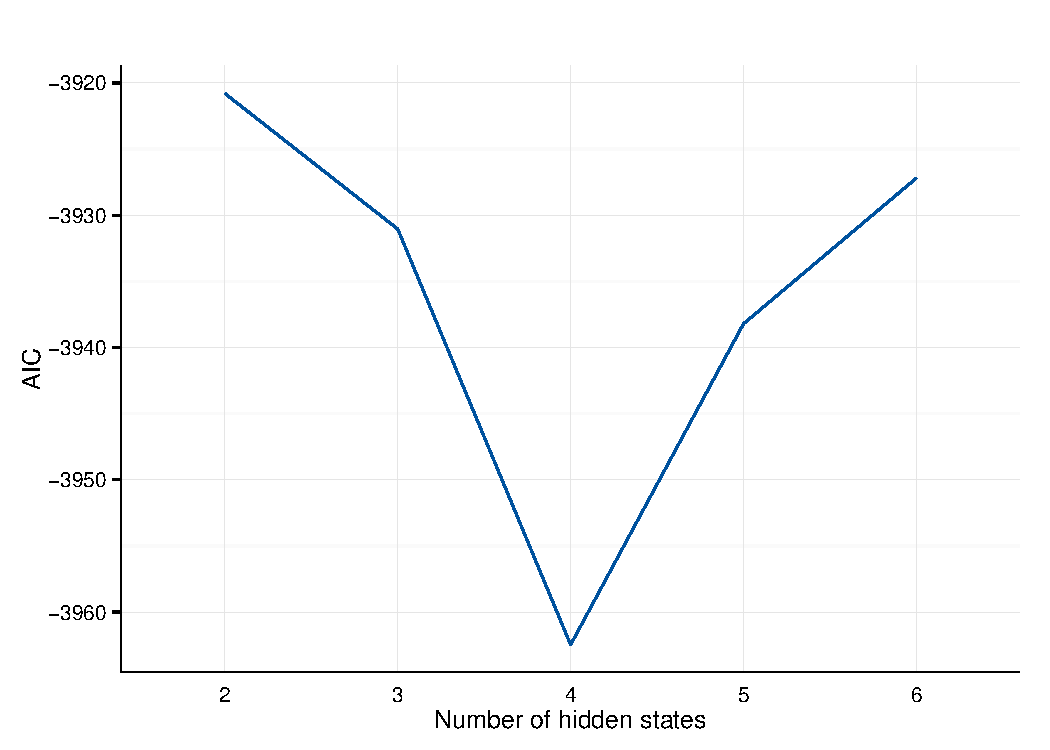
\includegraphics[width=0.45\textwidth]{states/numStateAIC.pdf}}
        \subfigure[BIC vs. N]
            {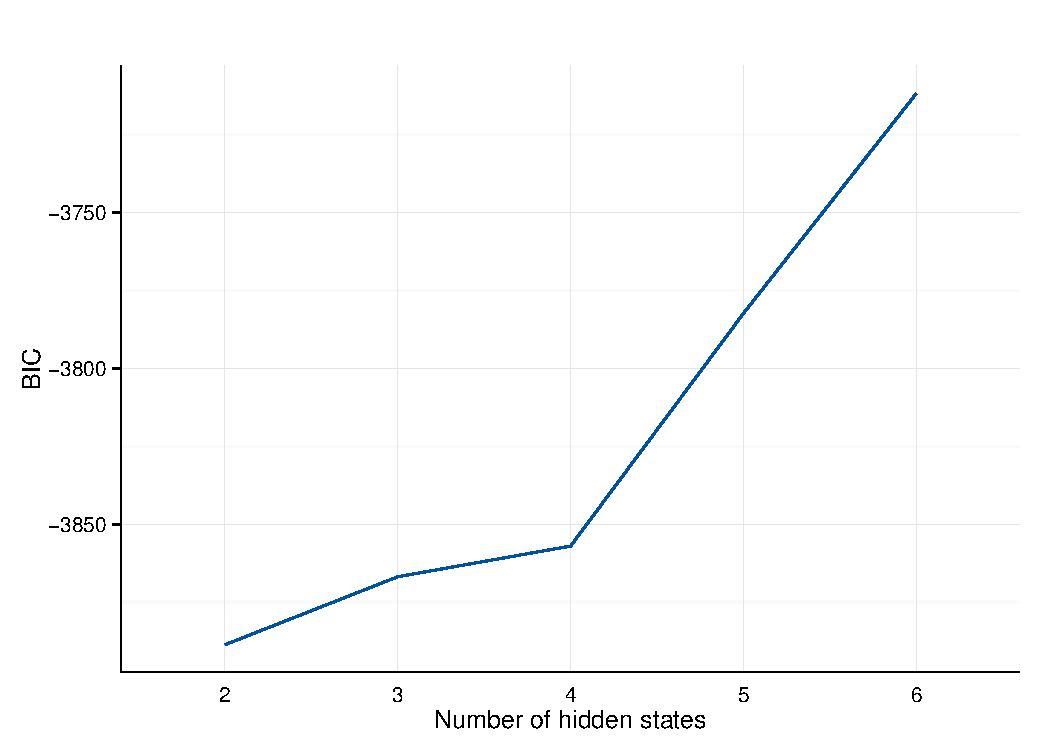
\includegraphics[width=0.45\textwidth]{states/numStateBIC.pdf}}
        \end{center}
        \caption{Goodness of fit for different number of hidden states}
        \label{fig:result:states}
        \end{figure}
We state in Assumption \ref{asp:states} that the markets have only three hidden states
and we name them as bear, intermediate and bull.
As is conventionally acknowledged, there are bull markets and bear markets.
However there are also intermediates that do not have obvious trends 
and fluctuations dominate during the period,
where only two states are not enough to describe the markets.
Certainly more market states could be introduced to the model 
(e.g.\,four to represent big rises, small rises, small falls and big falls),
but more states also bring higher risk of over-fitting and 
higher possibility to lack in realistic economic meanings.

Illus.\,\ref{fig:result:states} and Table \ref{table:result:states} indicate that 
two is the optimal parameter of 
the number of states based on BIC and four optimal according to AIC.
Thus we choose three as the parameter, 
which is the most widely used (see \cite{Zucchini:2009df,Dias:2015ky,Nystrup:2015ic}),
statistically (nearly) optimal and also economically meaningful.
Yet still the reader should notice that it is possible there are more optimal parameter selections.

        \begin{table}[!hbt]
        \center
        \caption{Numerical results of goodness of fit for different number of states}
        \label{table:result:states}
        \begin{tabular}{c c c}
        \hline
        Number of States  &  \hspace*{5em}AIC\hspace*{5em}  &  \hspace*{5em}BIC\hspace*{5em} \\
        \hline
        2   &   -3920.80    &   -3888.71    \\
        3   &   -3931.05    &   -3866.86    \\
        4   &   -3962.47    &   -3857.02    \\
        5   &   -3938.21    &   -3782.33    \\
        6   &   -3927.20    &   -3711.71    \\
        \hline
        \end{tabular}
        \end{table}

